\section{Comparison of Existing Alternative Games}
\label{chap:comparison_of_existing_games}

To compare the alternative aspects of all the games mentioned in the previous chapter, the alternative games model presented in Chapter \ref{chap:what_is_alternative_game} has been used. It provides a quick overview of how the game differs and presents concrete characteristics for all the games in each of the six categories. The model in Table \ref{tab:existing_games} is a simplified version of the complete model found in Appendix \ref{appendix:complete_model} where the unused rows have been omitted for readability.
\begin{table}[H]
    \vspace*{-0.4\baselineskip}
    \centering
    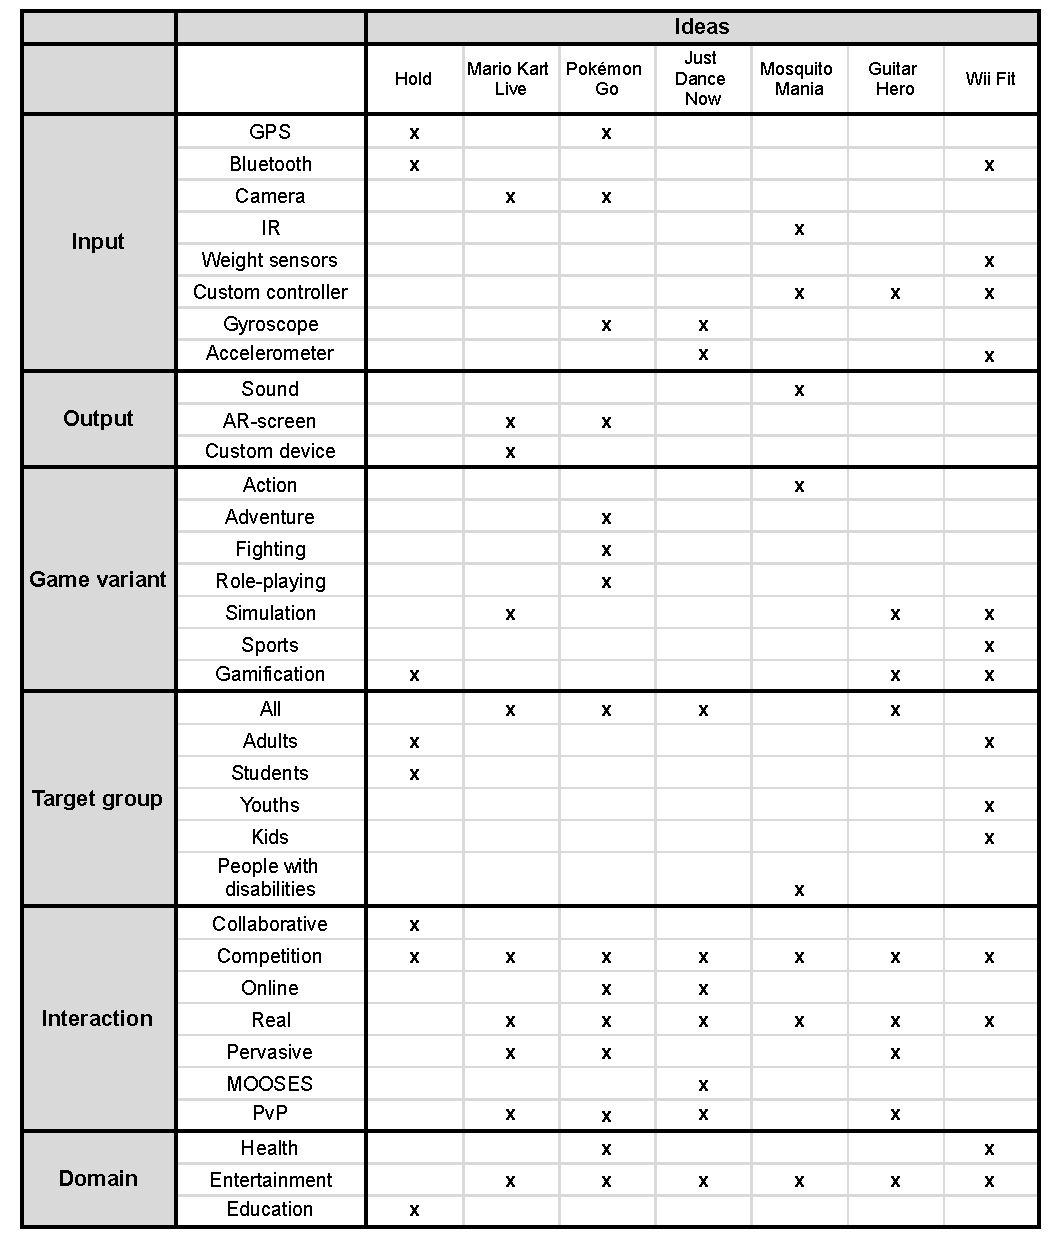
\includegraphics[width=0.92\textwidth]{Images/Models/ExistingGames.pdf}
    \caption{Existing alternative games characteristics}
    \label{tab:existing_games}
    \vspace*{-\baselineskip}
\end{table}


\subsection{Analysis of Input}
The first section of the model shows a wide range of \textit{input} types used in the games.  The variation is likely to come from the fact that many games are developed for a mobile platform. Mobile phones today include various input sensors that can be used to create alternative game concepts. GPS, Bluetooth, and gyroscopes are examples of such sensors. 

The games Hold, Pokémon Go, and Just Dance Now are totally or partially developed for mobile platforms. Hold and Pokémon Go uses the device’s GPS to use the context of the player’s location in the game. The location-aware feature creates a better in-game experience, and players are forced to move to unlock certain features. Pokémon Go and Just Dance Now both take advantage of the phone’s gyroscope. The gyroscope can detect rotation, telling a game how the mobile device is positioned in the real world. Just Dance Now also uses the accelerometer to track the player’s movement while dancing. The use of both gyroscope and accelerometer determines if the player is doing the right move at the right time, providing a fun and immersive player experience.

In the early days of computer games, custom controllers for each game were common \citep{overmars_brief_2012}. Using different controllers was adverse for the players because it forced them to buy new ones for every game. Furthermore, non-custom controllers can cause a poor user experience if it does not have an optimal or logical design. Nowadays, custom controllers are rare, and games are often produced for specific consoles rather than unique controllers. However, there exist games today with custom controllers, and Guitar Hero, Wii Fit, and Mosquito Mania are all examples of this. In these games, it makes sense to use a custom controller more suited for the game's purpose since a regular game controller would make it hard to create a realistic game. Using a special controller as input is a classic example of an alternative game.

\subsection{Analysis of Output}
The second section of the model looks at the alternative use of \textit{output} in games. Even though today’s games often use sound effects and music, this does not make them alternative. The use of sound in Mosquito Mania is more alternative as it is the only output. The game focuses on the player's ability to sense the sound's direction, which is an alternative way of challenging the player's hearing instead of the eyesight.

Furthermore, Pokémon Go and Mario Kart Live use the camera as an input to produce an Augmented Reality (AR) output. AR technology is alternative in games because projecting artificial objects onto the real world is based on interpreted input. In both games, players use a handheld device. AR in mobile devices is more available to the consumers but creates a less immersive gaming experience than an AR headset.

\subsection{Analysis of Game Variant}
A selection of \textit{game variants} is listed in the third section of the table. These game variants themself do not make games alternative; although, they do tell something about what type of game it is. There is one exception to this: gamification. Gamification is alternative because it uses game design principles to make activities and tasks fun and engaging while motivating the player. Hold, Guitar Hero, and Wii Fit are all gamification concepts. Hold gamifies and rewards players for putting the phone down, Guitar Hero gamifies playing the guitar, and Wii Fit gamifies and motivates working out. Furthermore, games can also be classified within several variants, making the game more alternative, though this is not implied.

\subsection{Analysis of Target Group}
The identified \textit{target groups} can be found in the fourth section of the model. All games have one or more dedicated target groups, corresponding to everyone or a distinguished set of users. The target groups might overlap or intersect; for instance, students and young adults intersect. Mario Kart Live, Just Dance Now, and Guitar Hero are examples of games where the target group is “all”. Still, these games might be more addressed towards a younger crowd. Mosquito Mania is also a game that most people can play; however, it is especially applicable for people with visual impairment who may have trouble playing ordinary games.

\subsection{Analysis of Interaction}
The fifth section of the model displays the types of \textit{interactions} that have been identified in the existing games studied in Chapter \ref{chap:existing_games}. Interaction types can be found in all ordinary games and do not imply that a game is alternative. However, how the interaction is accomplished may be categorized as alternative. All seven games use a combination of interaction methods, and all games include some degree of interaction through competition. Competition can be conducted in numerous ways, e.g., by utilizing a scoreboard. Just Dance Now offers, like many other games, different player modes. Players can play alone, against friends in the same physical or virtual room in real-time, or online through the global scoreboard. These gameplay variations make the game very flexible, and players can play in the way they want. The other games offer similar but not so extensive features as Just Dance Now. Mario Kart Live, Pokémon Go, and Guitar Hero all include the competitive elements of PvP interaction. In these games, players communicate in the real world, but the gameplay happens in the virtual world.

Hold is the only game that includes a collaborative mode where players can connect their device with their friends’ to boost points. If one player quits, the player will not only lose his or her focus but also stop the boosting for the collaborating players. This interaction feature is likely to strengthen the player’s motivation for not using their phones. 

\subsection{Analysis of Domain}
The sixth and last section of the model displays the \textit{domain} of the games. Traditionally speaking, games often belong to the domain of entertainment, and therefore the use of other domains can classify a game as alternative. The exercise game Wii Fit is directly connected to the domain of physical health. Pokémon Go also exploits the benefits of physical health from having players move around. Hold is not like a traditional game and thus classifies only in the educational domain since its primary target group is students.

\subsection{Summary}
This chapter has focused on showcasing multiple different and typical examples of alternative games (based on our definition presented in Chapter \ref{chap:what_is_alternative_game}). The examples have been shortly described and compared with each other to highlight their differences. A table with the characteristics of each game has been presented and analyzed. The next chapter will shift the focus from the concept to the technical aspect of alternative games.  
